% ============================================================
% Anonymous conference-facing manuscript
% Scientific state: closed Pilot B plus frozen post-closure diagnostic
% Detailed development and audit record: separate supplementary material
% 27 August 2026
% ============================================================

\documentclass[runningheads]{llncs}

\usepackage[T1]{fontenc}
\usepackage[utf8]{inputenc}
\usepackage{amsmath,amssymb,amsfonts}
\usepackage{booktabs}
\usepackage{tabularx}
\usepackage{tikz}
\usetikzlibrary{arrows.meta,positioning}
\usepackage{hyperref}

\hypersetup{hidelinks}

\newcommand{\SHAP}{SHAP}
\newcommand{\XGB}{XGBoost}
\newcommand{\MOORA}{MOORA}
\newcommand{\CRITIC}{CRITIC}
\newcommand{\E}{\mathbb{E}}
\newcommand{\I}{\mathbb{I}}
\newcommand{\median}{\operatorname{median}}

\begin{document}
\emergencystretch=1.5em

\title{Do Global XAI--MCDM Weights Add Decision Value?\\
A Prospectively Gated ITS Benchmark Study}
\titlerunning{Prospectively Gated Global XAI--MCDM Benchmark}

\author{Anonymous Author(s)}
\authorrunning{Anonymous Author(s)}
\institute{Anonymous institution(s)}

\maketitle

\begin{abstract}
Machine-learning explanations are increasingly converted into global criterion weights and
then used in multi-criteria decision-making, but predictive attribution does not guarantee a
better decision. We ask a prior question: is a controlled benchmark sufficiently
discriminative to support that comparison? We construct a synthetic Intelligent
Transportation Systems laboratory with six alternatives, ten criteria, a nonlinear oracle,
\XGB, interventional TreeSHAP, six structured global-weight pipelines and benefit-oriented
\MOORA. Structural diagnostics first exposed an initial generator whose apparent contextual
variation cancelled under within-context normalization. A corrected monotone kernel removed
that algebraic defect, after which a prospectively frozen five-world gate tested decision value
at one authorized development condition. All six structured methods were eligible. Four methods,
including SHAP, materially outperformed RandomWeights; SHAP attained median
$\Delta\tau_b=0.288$ with positive advantage in all five worlds. Nevertheless, no method---not
even closed-form oracle attribution under the frozen interventional functional---reliably
outperformed a world-specific constant MajorityWinner under the prespecified median-margin and
four-of-five consistency rule. SHAP's median Top-1 and regret advantages over that reference
were both zero. A separately frozen post-closure diagnostic reconstructed 7000 context-level
selections: Equal-weight \MOORA was constant in all five worlds and exactly matched
MajorityWinner in four, whereas structured-method constancy ranged from zero to three worlds.
The gate therefore barred the planned primary factorial. This condition-specific negative
result does not show that SHAP, global weights or \MOORA fail generally. It shows why synthetic
XAI--MCDM studies should establish downstream decision discrimination against meaningful
simple references before claiming comparative method performance.

\keywords{Explainable AI \and Multi-Criteria Decision-Making \and Benchmark Validity \and
Prospective Stopping \and Decision Support \and Intelligent Transportation Systems}
\end{abstract}

% ============================================================
\section{Introduction}
\label{sec:introduction}
% ============================================================

Transport agencies often need to prioritise Intelligent Transportation Systems (ITS) with
limited operational evidence and limited capacity for formal preference elicitation. The task
is naturally multi-criteria: alternatives can differ in mobility, reliability,
person-throughput, safety, environmental performance, accessibility, readiness,
interoperability and lifecycle burden. Machine learning and explainable artificial intelligence
(XAI) offer an apparently attractive shortcut: learn a performance model, aggregate feature
attributions into criterion ``importance'', normalize them into weights and rank alternatives
with a multi-criteria decision-making (MCDM) rule.

That shortcut contains a semantic and an empirical leap. MCDM weights acquire meaning from the
criterion scales and aggregation model; they are not generic measures of importance
\cite{keeney1976decisions,roy1996importance,choo1999weights}. SHAP values allocate model output
under a specified cooperative-game functional \cite{lundberg2017shap}, but the resulting
predictive attribution is not automatically a stakeholder preference, causal effect or valid
trade-off constant \cite{sundararajan2020many,kumar2020shapleyproblems,janzing2020causal}.
Consequently,
\[
\text{predictive attribution}
\longrightarrow
\text{global criterion weight}
\longrightarrow
\text{MCDM ranking}
\]
is a pipeline to validate, not an identity to assume.

Controlled synthetic studies appear well suited to this validation because the data-generating
process and an oracle reference are known. Yet a synthetic benchmark can contain substantial raw
variation while still producing nearly invariant normalized decision matrices or highly
concentrated choices. In that situation, an elaborate comparison can measure implementation
differences without asking a genuinely discriminative decision question. Benchmark studies are
also vulnerable to over-optimism when generators, estimands or analyses are revised after
method performance is observed \cite{morris2019simulation,niessl2022overoptimism}.

We address three research questions:

\begin{description}
\item[RQ1.] Can structural diagnostics reveal when contextual variation disappears under the
normalization used by the downstream MCDM operator?
\item[RQ2.] After correcting that defect, do structured global-weight pipelines provide enough
incremental decision value over random-weight and constant-decision references to justify a
larger comparison?
\item[RQ3.] What does the observed context-level decision map reveal about the stopped result?
\end{description}

The paper contributes a compact validation workflow rather than a new weighting algorithm.
First, it separates raw variation, structural non-separability and decision discrimination.
Second, a closed-form attribution reference helps distinguish errors in learned SHAP from losses
created by global compression and MCDM. Third, a prospectively frozen adequacy gate prevents the
planned primary comparison from running when its decision premise fails. The full generator
genealogy, candidate grids, seed namespaces, software tests, frozen protocols and unexecuted
analyses are preserved in the companion supplement; they establish reproducibility without
making the audit trail the main research story.

Figure~\ref{fig:workflow} gives the complete study logic. The separation between estimation and
external TEST, the parallel oracle reference and the final prospective gate are central: a
pipeline is evaluated by the decisions it induces, not by attribution similarity alone.

\begin{figure}[t]
\centering
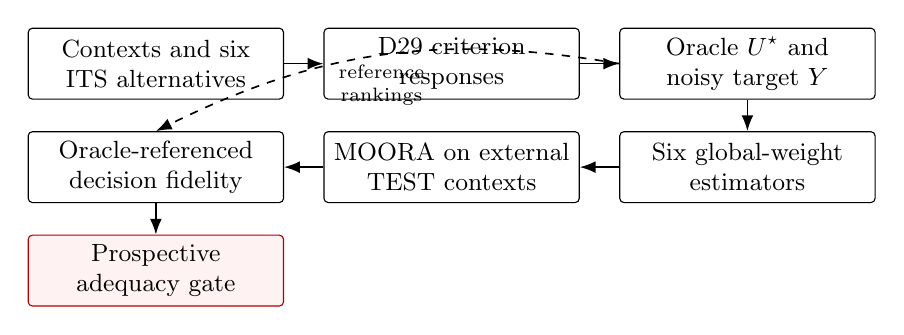
\begin{tikzpicture}[
  node distance=4mm and 5mm,
  box/.style={draw, rounded corners=1.5pt, align=center, minimum height=9mm,
              text width=.25\linewidth, inner sep=3pt, font=\small},
  gate/.style={draw=red!70!black, fill=red!5, rounded corners=1.5pt, align=center,
               minimum height=9mm, text width=.25\linewidth, inner sep=3pt, font=\small},
  arr/.style={-{Latex[length=2mm]}, semithick}
]
\node[box] (context) {Contexts and six\\ITS alternatives};
\node[box, right=of context] (responses) {D29 criterion\\responses};
\node[box, right=of responses] (oracle) {Oracle $U^\star$ and\\noisy target $Y$};
\node[box, below=of oracle] (weights) {Six global-weight\\estimators};
\node[box, left=of weights] (moora) {\MOORA\ on external\\TEST contexts};
\node[box, left=of moora] (fidelity) {Oracle-referenced\\decision fidelity};
\node[gate, below=of fidelity] (adequacy) {Prospective\\adequacy gate};
\draw[arr] (context) -- (responses);
\draw[arr] (responses) -- (oracle);
\draw[arr] (oracle) -- (weights);
\draw[arr] (weights) -- (moora);
\draw[arr] (moora) -- (fidelity);
\draw[arr] (fidelity) -- (adequacy);
\draw[arr,dashed] (oracle.west) to[bend right=18]
  node[below, font=\scriptsize, align=center] {reference\\rankings} (fidelity.north);
\end{tikzpicture}
\caption{Conference-level workflow. FIT/WEIGHT data support model fitting and global-weight
estimation; independent TEST contexts support \MOORA\ decisions and oracle-referenced fidelity.
The gate decides whether the protected primary comparison is scientifically warranted.}
\label{fig:workflow}
\end{figure}

% ============================================================
\section{Related Work and Contribution Boundary}
\label{sec:related}
% ============================================================

Existing XAI--MCDM studies demonstrate that model explanations can be integrated with ranking
methods in application domains including transport and infrastructure
\cite{ciano2025xaimcdm,demir2025shapmultimoora,zakeri2024mlmcdm}. Objective weighting methods
such as \CRITIC\ and entropy instead use dispersion and conflict in a decision matrix
\cite{diakoulaki1995critic,shannon1948,mukhametzyanov2021objective}. These methods answer
different questions: attribution-based methods summarize a predictive functional; regression
and permutation methods use supervised association; and objective weights summarize the
observed criterion matrix. Their numerical outputs are therefore not interchangeable notions of
preference.

Synthetic XAI benchmarks compare explanations with known targets
\cite{liu2021xaibench,agarwal2022openxai}. Our focus is downstream: even exact recovery of a
global attribution functional need not recover context-specific oracle choices after
compression into one fixed vector and aggregation. The distinction matters because prediction,
attribution and decision fidelity can fail at different stages. We therefore compare learned
SHAP with a matched closed-form oracle attribution and evaluate both using ranking, Top-1 and
regret metrics.

The contribution boundary is deliberately narrow. This study does not estimate empirical ITS
effects, elicit stakeholder preferences, identify a preferred real-world intervention, or test
whether SHAP works universally. ITS provides a controlled applied decision setting. The
scientific object is the validity of a global-weight XAI--MCDM benchmark at one prospectively
specified development reference.

% ============================================================
\section{Benchmark and Validation Design}
\label{sec:methods}
% ============================================================

\subsection{ITS Decision Laboratory}

The benchmark compares six deployment packages at a common first-stage prioritisation level
(Table~\ref{tab:alternatives}). They represent deployable ITS/transport-systems-management
families rather than calibrated effects for a particular city
\cite{fhwa2016corridors,fhwa2017atm,usdotv2x}.

\begin{table}[t]
\centering
\caption{ITS alternatives in the controlled decision laboratory.}
\label{tab:alternatives}
\small
\begin{tabularx}{\linewidth}{@{}c l X@{}}
\toprule
\textbf{ID} & \textbf{Alternative} & \textbf{Operational scope}\\
\midrule
$A_1$ & ATSC & Adaptive phase, split, offset or cycle decisions.\\
$A_2$ & TSP & Transit-priority requests and signal responses.\\
$A_3$ & TIDM & Incident detection, verification, response and recovery.\\
$A_4$ & RMTI--DRG & Real-time multimodal information and dynamic route guidance.\\
$A_5$ & V2X--CS & Cooperative safety warnings, excluding signal timing and TSP.\\
$A_6$ & DSM & Dynamic speed management and harmonisation.\\
\bottomrule
\end{tabularx}
\end{table}

Ten benefit-oriented criteria describe mobility efficiency, reliability, person-throughput,
safety, resilience, environmental efficiency, accessibility, readiness,
interoperability/scalability and direction-adjusted lifecycle burden. Five correlated latent
factors describe demand, incidents, person movement, environmental sensitivity and
infrastructure readiness. Each replication seed defines a complete benchmark world---including
technology parameters, contexts and random streams---and is the statistical unit. Alternative--
context rows are not treated as independent population replications.

\subsection{Structural Defect and Frozen Correction}
\label{sec:generator}

The initial noise-free response for active criteria $C_1$--$C_7$ had the form
\begin{equation}
g_{asj}=\theta_{aj}o_{sj},
\label{eq:separable}
\end{equation}
where $a$, $s$ and $j$ index alternative, context and criterion. Under vector normalization,
\begin{equation}
r_{asj}
=\frac{\theta_{aj}o_{sj}}{\sqrt{\sum_b\theta_{bj}^2o_{sj}^2}}
=\frac{\theta_{aj}}{\sqrt{\sum_b\theta_{bj}^2}},
\label{eq:collapse}
\end{equation}
for $o_{sj}>0$. Thus raw contextual variation cancels exactly. Sum, max and min--max
normalizations have the analogous common-scale cancellation. This is the answer to RQ1: raw
variation alone was not evidence of a context-sensitive decision benchmark.

After prospectively separated calibration and eligibility checks, the frozen D29 correction for
active $C_1$--$C_7$ pathways was
\begin{equation}
g_{asj}=\theta_{aj}o_{sj}+0.05v_{aj}o_{sj}(1-o_{sj}),
\qquad v_{aj}\in[-1,1].
\label{eq:d29}
\end{equation}
The deterministic $v_{aj}$ values were created without outcome or winner information. Because
$\theta_{aj}\geq0.05$, the response remains monotone on $o\in[0,1]$. D29 was retained for
protocol continuity and minimal intervention among 54 corrected-eligible candidates, not
because it produced a preferred ITS winner or favourable method comparison. The full rejected
family and candidate history are supplementary.

\subsection{Oracle, Global Weights and Decision Operator}

Benefit-oriented criterion values are mapped by
$q_j(g)=\log(1+2g)/\log 3$. The noise-free oracle is
\begin{equation}
U_{as}^{\star}
=\frac{\sum_{j=1}^{10}\alpha_jq_j(g_{asj})
+\lambda\sum_{(j,k)\in\mathcal E}0.20\,q_j(g_{asj})q_k(g_{ask})}
{1+\lambda}.
\label{eq:oracle}
\end{equation}
This is an internally specified reference, not causal truth or social welfare. The prediction
target adds controlled noise to $U^\star$. Because Eq.~\eqref{eq:oracle} contains main effects
and pairwise interactions, the frozen interventional Shapley functional has a closed-form oracle
attribution. Global oracle weights normalize mean absolute WEIGHT-set attributions. Learned SHAP
uses the same aggregation on interventional TreeSHAP values from a fixed \XGB\ model
\cite{chen2016xgboost,lundberg2020trees}.

Six structured global-weight methods enter the gate: oracle attribution, SHAP, fixed-model
context-block permutation importance (PI), non-negative Ridge+, \CRITIC\ and entropy. Equal,
RandomWeights and MajorityWinner are diagnostic references. Every weighting method produces one
context-invariant vector per world. Estimation uses disjoint FIT and WEIGHT partitions; the 200
external TEST contexts are never used for fitting or weight estimation. At Pilot B's
$N=250$, each world contains 200 FIT contexts, 50 WEIGHT contexts and 200 TEST contexts.

The downstream operator is benefit-oriented weighted \MOORA\ \cite{brauers2006moora}:
\begin{equation}
r_{asj}=\frac{g_{asj}}{\sqrt{\sum_{b=1}^{6}g_{bsj}^2}+10^{-12}},
\qquad
S_{as}=\sum_{j=1}^{10}w_jr_{asj}.
\label{eq:moora}
\end{equation}
Alternatives are ranked by descending $S_{as}$. All score representations use an absolute
$10^{-12}$ tie tolerance, anchor-based average ranks without tie chaining, and ascending
alternative ID for deterministic Top-1 selection.

\subsection{Decision Fidelity and the Prospective Gate}

We measure full-ranking agreement with oracle $U^\star$ using Kendall's $\tau_b$, deterministic
Top-1 accuracy, and normalized oracle regret
\begin{equation}
R_s^{(q)}=
\frac{U_{a_s^\star,s}^{\star}-U_{\hat a_s^{(q)},s}^{\star}}
{\max_aU_{as}^{\star}-\min_aU_{as}^{\star}+10^{-12}}.
\label{eq:regret}
\end{equation}

Pilot B was frozen before execution at
$(N,c,\rho,\lambda)=(250,0.30,0.4,0.5)$ for development worlds 21001--21005. It uses 200 common
$\operatorname{Dirichlet}(1,\ldots,1)$ RandomWeights draws and one MajorityWinner per world.
MajorityWinner is the oracle-modal constant alternative estimated on WEIGHT and evaluated on
TEST. It is an oracle-informed diagnostic, not an operational competitor and not necessarily the
minimum-regret constant policy.
The comparison is deliberately conservative: a global-weight pipeline must add decision value
beyond this simple constant-choice rule before its additional methodological complexity is
considered justified.

A practical method advantage must be strictly positive in at least four of five worlds and meet
the relevant cross-world median margin. Table~\ref{tab:gates} summarizes the five independently
sufficient stops. The overall rule is an OR: the benchmark passes only if every stop is false.
The margins are design-specific adequacy tolerances, not universal equivalence bounds.

\begin{table}[t]
\centering
\caption{Prospectively frozen Pilot-B stop conditions.}
\label{tab:gates}
\small
\begin{tabularx}{\linewidth}{@{}l X@{}}
\toprule
\textbf{Stop} & \textbf{Condition}\\
\midrule
Coverage & A required structured output or RandomWeights coverage is missing.\\
Random equivalence & No method clears median $\Delta\tau_b=0.05$ or
$\Delta$mean-regret $=0.01$ versus RandomWeights.\\
Modal-winner tie & No method clears median $\Delta$Top-1 $=0.02$ or
$\Delta$mean-regret $=0.01$ versus MajorityWinner.\\
Oracle dominance & Pooled oracle modal share is at least $0.90$.\\
Weight insensitivity & Random-weight choices or performance widths meet the frozen invariance
criteria.\\
\bottomrule
\end{tabularx}
\end{table}

The protocol, evaluator and protected seed firewall were committed before the single authorized
execution. A 30-world, 135-cell factorial and associated robustness analyses were conditional on
Pilot-B passage. They were not run. This is version-controlled prospective specification rather
than public preregistration; complete provenance appears in the supplement.

% ============================================================
\section{Results}
\label{sec:results}
% ============================================================

\subsection{Structural Validity Did Not Guarantee Decision Diversity}

The historical generator in Eq.~\eqref{eq:separable} showed numerical collapse exactly where
the algebra predicted it: across 35 world--criterion combinations, the maximum active-pair log-
ratio variation was $7.2224\times10^{-16}$ and maximum vector-normalized profile variation was
$1.8036\times10^{-9}$. The corrected D29 kernel passed the frozen structural and reachability
requirements, but its oracle decision geometry remained heterogeneous (Table~\ref{tab:d29}).

\begin{table}[t]
\centering
\caption{Frozen D29 oracle-side diagnostics over 1000 development contexts per world. Regret is
for the always-modal oracle winner.}
\label{tab:d29}
\small
\begin{tabular}{@{}r r r r r@{}}
\toprule
World & Orderings & Winners & Modal share & Mean regret\\
\midrule
21001 & 23 & 2 & 0.983 & 0.00042018\\
21002 & 78 & 5 & 0.519 & 0.05992337\\
21003 & 24 & 4 & 0.745 & 0.04523642\\
21004 & 17 & 3 & 0.827 & 0.01734351\\
21005 & 38 & 4 & 0.809 & 0.01606539\\
\bottomrule
\end{tabular}
\end{table}

D29 produced multiple oracle orderings and winners in every world, yet modal share ranged from
$0.519$ to $0.983$. In the directly comparable world 21001, the correction increased distinct
oracle orderings from 19 to 23 relative to the historical generator but increased modal share
from $0.962$ to $0.983$. Removing exact multiplicative separability was therefore necessary for
this benchmark, but it did not guarantee a broadly discriminative decision frontier.

\subsection{Pilot B Stopped the Primary Comparison}
\label{sec:pilotb}

All six structured methods were defined in every world, all required Kendall summaries were
available and no Equal fallback was used. Table~\ref{tab:gateoutcome} gives the independently
reconstructed gate decision. Four of six methods separated from RandomWeights, so the random-
equivalence stop was false. The pooled oracle modal share was $0.526$ (A2 in 526 of 1000 TEST
contexts), so no single alternative dominated the pooled worlds. RandomWeights decisions were
also not invariant. Only the modal-winner effective-tie stop fired.

\begin{table}[t]
\centering
\caption{Frozen Pilot-B outcome. The overall hard stop is the OR of the five flags.}
\label{tab:gateoutcome}
\small
\begin{tabularx}{\linewidth}{@{}lXc@{}}
\toprule
Gate & Audited result & Stop\\
\midrule
Coverage & Six structured methods eligible without fallback & No\\
Random equivalence & Four of six methods separated from RandomWeights & No\\
Modal-winner tie & Zero of six methods escaped MajorityWinner & \textbf{Yes}\\
Oracle dominance & Pooled modal share $0.526<0.90$ & No\\
Weight insensitivity & Invariant fraction $0.004<0.90$; qualified worlds $0<4$ & No\\
\midrule
Overall & At least one prospectively frozen stop fired & \textbf{Yes}\\
\bottomrule
\end{tabularx}
\end{table}

Table~\ref{tab:contrasts} localizes the failure. Positive values favour the structured method.
Oracle attribution, SHAP, PI and Ridge+ all cleared a RandomWeights criterion with the required
cross-world consistency. SHAP showed the largest median Kendall improvement, $0.288$, positive
in all five worlds, and a median regret improvement of $0.026060$, positive in four. Against
MajorityWinner, however, its median Top-1 and regret advantages were both exactly zero, with only
two positive worlds. No method met either modal-winner margin with the required four-of-five
consistency.

\noindent\textbf{Takeaway.} SHAP preserved structured decision-ranking information relative to
random weights, but global-weight compression and \MOORA\ did not convert that information into
sufficient incremental choice value at the frozen reference condition.

\begin{table}[t]
\centering
\caption{Cross-world median Pilot-B contrasts with strict positive-world counts (P). MW denotes
MajorityWinner and RW denotes RandomWeights.}
\label{tab:contrasts}
\scriptsize
\setlength{\tabcolsep}{2.5pt}
\begin{tabular}{@{}lrrrrc@{}}
\toprule
Method & \shortstack{MW\\$\Delta$Top-1 (P)} & \shortstack{MW\\$\Delta$regret (P)} &
\shortstack{RW\\$\Delta\tau_b$ (P)} & \shortstack{RW\\$\Delta$regret (P)} & RW sep.\\
\midrule
Oracle attribution & $-0.010$ (1) & $-0.002119$ (1) & $0.209$ (5) & $0.023940$ (4) & Yes\\
SHAP & $0.000$ (2) & $0.000000$ (2) & $0.288$ (5) & $0.026060$ (4) & Yes\\
Permutation importance & $-0.120$ (1) & $-0.004425$ (1) & $0.194$ (5) & $0.010658$ (4) & Yes\\
Ridge+ & $-0.010$ (1) & $-0.002119$ (1) & $0.237$ (5) & $0.011492$ (4) & Yes\\
CRITIC & $-0.580$ (0) & $-0.124414$ (0) & $0.030$ (3) & $-0.098354$ (0) & No\\
Entropy & $-0.580$ (0) & $-0.156641$ (0) & $0.035$ (3) & $-0.002807$ (1) & No\\
\bottomrule
\end{tabular}
\end{table}

\begin{figure}[t]
\centering
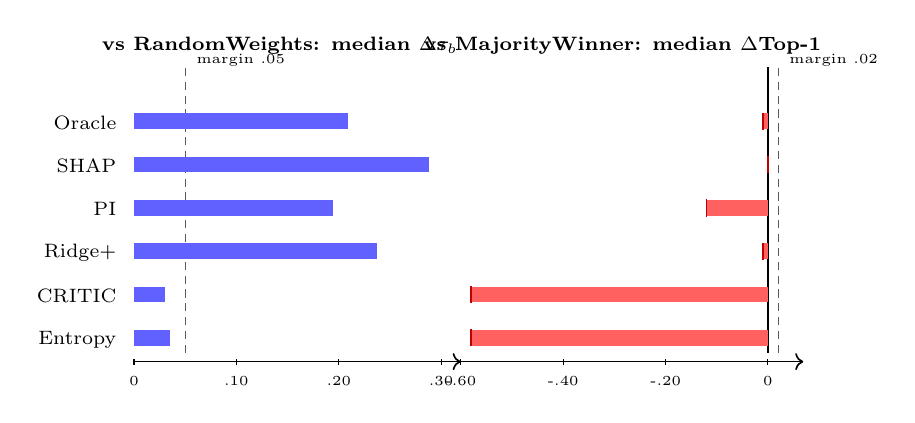
\begin{tikzpicture}[x=1cm,y=0.55cm]
  \node[font=\scriptsize\bfseries] at (1.85,6.75)
    {vs RandomWeights: median $\Delta\tau_b$};
  \draw[->,semithick] (0,-0.55) -- (4.15,-0.55);
  \foreach \x/\lab in {0/0,1.3/.10,2.6/.20,3.9/.30}{
    \draw (\x,-0.62) -- (\x,-0.48);
    \node[font=\tiny,anchor=north] at (\x,-0.68) {\lab};
  }
  \draw[densely dashed,black!65] (0.65,-0.35) -- (0.65,6.25);
  \node[font=\tiny,anchor=south west] at (0.67,6.05) {margin .05};
  \foreach \name/\yy/\rw in {
    Oracle/5/0.209,SHAP/4/0.288,PI/3/0.194,Ridge+/2/0.237,
    CRITIC/1/0.030,Entropy/0/0.035}{
      \node[font=\scriptsize,anchor=e] at (-0.10,\yy) {\name};
      \fill[blue!62] (0,\yy-0.18) rectangle ({13*\rw},\yy+0.18);
  }
  \begin{scope}[xshift=8.05cm]
    \node[font=\scriptsize\bfseries] at (-1.85,6.75)
      {vs MajorityWinner: median $\Delta$Top-1};
    \draw[->,semithick] (-4.05,-0.55) -- (0.45,-0.55);
    \foreach \x/\lab in {-3.9/-.60,-2.6/-.40,-1.3/-.20,0/0}{
      \draw (\x,-0.62) -- (\x,-0.48);
      \node[font=\tiny,anchor=north] at (\x,-0.68) {\lab};
    }
    \draw[semithick] (0,-0.35) -- (0,6.25);
    \draw[densely dashed,black!65] (0.13,-0.35) -- (0.13,6.25);
    \node[font=\tiny,anchor=south west] at (0.15,6.05) {margin .02};
    \foreach \yy/\mw in {5/-0.010,4/0.000,3/-0.120,2/-0.010,1/-0.580,0/-0.580}{
      \fill[red!62] (0,\yy-0.18) rectangle ({6.5*\mw},\yy+0.18);
      \draw[red!75!black,semithick]
        ({6.5*\mw},\yy-0.20) -- ({6.5*\mw},\yy+0.20);
    }
  \end{scope}
\end{tikzpicture}
\caption{The decisive contrast. Four structured methods exceeded the RandomWeights Kendall
margin (left), but no method reached the MajorityWinner Top-1 margin (right).}
\label{fig:contrast}
\end{figure}

This is more informative than saying that the methods were simply broken. Structured weighting
recovered reproducible ranking information relative to random weights. It did not convert that
information into reliable incremental Top-1 or regret value beyond the stronger constant-
decision diagnostic. The exact oracle-attribution reference also failed the gate, so the stop
cannot be attributed solely to \XGB\ fitting or SHAP approximation.

\subsection{Frozen Post-Closure Selection Maps}
\label{sec:selectionmaps}

The original Pilot-B result retained aggregate metrics but not method-level context selections.
After permanent closure, a separate protocol was frozen before reconstructing these selections.
It reused the archived fixed weights and TEST identities, generated no target, fitted or queried
no model, re-estimated no weight, and could not alter the gate. Its independent audit verified
all $5\times7\times200=7000$ selections.

Equal-weight \MOORA\ selected one alternative in every context of every world and exactly
matched MajorityWinner in four worlds (Table~\ref{tab:selectionmaps}). Structured-method
constancy ranged from zero worlds for PI to three for entropy, refuting universal fixed-weight
invariance among the observed vectors.

\begin{table}[t]
\centering
\caption{Post-closure diagnostic for the seven observed fixed vectors. Counts give worlds with
one selected alternative and worlds with exact context-level agreement with MajorityWinner.}
\label{tab:selectionmaps}
\small
\begin{tabular}{@{}lrr@{}}
\toprule
Method & Constant-selection worlds & All-context MW-match worlds\\
\midrule
Oracle attribution & 1/5 & 1/5\\
SHAP & 2/5 & 2/5\\
Permutation importance & 0/5 & 0/5\\
Ridge+ & 1/5 & 1/5\\
CRITIC & 2/5 & 1/5\\
Entropy & 3/5 & 2/5\\
Equal & 5/5 & 4/5\\
\bottomrule
\end{tabular}
\end{table}

World 21003 clarifies why Top-1 and full-ranking fidelity must be separated. Equal, \CRITIC\ and
entropy all selected A6 in all 200 contexts, giving identical Top-1 accuracy $0.190$ and mean
regret $0.316758$. Their mean $\tau_b$ values nevertheless differed ($0.5493$, $0.5427$ and
$0.5113$) because lower-ranked alternatives differed. This observed coincidence supports a
hypothesis of locally coarse decision regions for particular fixed vectors; it does not
characterize unobserved weight space or establish the cause of the Pilot-B stop.

% ============================================================
\section{Discussion}
\label{sec:discussion}
% ============================================================

\subsection{What the Study Establishes}

The results answer the three research questions directly. For RQ1, an algebraic and numerical
audit showed that context variation can disappear under the normalization used by the decision
operator. For RQ2, correcting exact separability produced multiple oracle orderings and winners,
but did not establish sufficient incremental decision value: no structured global-weight
pipeline escaped MajorityWinner under the frozen cross-world rule. For RQ3, the reconstructed
selection maps showed that Equal produced a constant decision in every world, while structured
vectors displayed heterogeneous constancy. The world-21003 result further demonstrated that
different full rankings can share the same context-invariant argmax.

The clearest interpretation is therefore not ``SHAP failed.'' SHAP was strongly separated from
RandomWeights, showing that its weights contained reproducible ranking information. Its entire
median advantage disappeared against MajorityWinner. At this reference, the bottleneck lay in
turning a single global weight vector into context-specific incremental decision value through
\MOORA. Closed-form oracle attribution reached the same negative gate outcome, which rules out
an explanation based solely on imperfect learned attribution. It does not isolate one causal
mechanism: generator geometry, global compression, reference construction and \MOORA\ geometry
remain coupled in the executed design.

For applied OR and transport studies, the practical lesson is simple. A complex data-driven
pipeline should be compared not only with random or uniform parameters but also with a meaningful
simple decision policy. Beating random weights can show that information was learned; it does not
show that the information changes the operational choice usefully. A prospective benchmark gate
can stop a large factorial before protected evaluations are consumed when that premise is not
met.

\subsection{Interpretation Boundary and Limitations}

The evidence covers five reused development worlds at one reference condition. It is a
condition-specific protocol screen, not independent population validation. It does not imply
that SHAP never works, that weights never matter, that \MOORA\ is generally inadequate, or that
one ITS alternative should be deployed. The synthetic capability mask, Gaussian copula,
response amplitudes and oracle are controlled assumptions rather than empirical transport
effects, causal truth, stakeholder preferences or social welfare.

Every global-weight method intentionally compresses context-specific information. The methods
also have different semantics: oracle attribution and SHAP target one interventional functional;
Ridge+ and PI use supervised associations; and \CRITIC\ and entropy summarize pooled decision-
matrix properties. PI can additionally extrapolate when dependence is broken
\cite{hooker2021permutation}. Their comparison evaluates downstream decision behavior, not
interchangeable estimates of normative importance.

The five-world consistency unit limits inferential precision. The original aggregate artefact
also omitted context-level method selections. The later frozen diagnostic repaired that
granularity for descriptive selection maps, but added no independent worlds. A paired context
bootstrap was prospectively excluded from that layer and was not executed; any resampling study
would require a separate protocol and could not reopen the gate. Likewise, the frozen margins
are design-specific adequacy tolerances rather than universal equivalence thresholds.

The negative result remains scientifically useful because it was not tuned away. The generator
correction, gate thresholds, evaluator and seed firewall preceded the authorized result. Once
the modal-winner stop fired, the 30-world primary factorial and reserve worlds remained barred.
Any future design must begin as a separately versioned study that acknowledges this closed
result rather than retroactively changing v1.

% ============================================================
\section{Conclusion}
\label{sec:conclusion}
% ============================================================

This study asked whether a synthetic ITS benchmark could support a global XAI--MCDM method
comparison before running the comparison at scale. Structural auditing found and corrected a
normalization-induced collapse, but the correction did not guarantee downstream decision
discrimination. At the frozen development reference, four structured methods---including
SHAP---clearly outperformed RandomWeights, yet none reliably improved on a world-specific
constant MajorityWinner. The exact attribution reference also failed this gate. A frozen
context-level diagnostic subsequently showed that Equal-weight \MOORA\ was constant in all five
worlds and matched MajorityWinner in four, while structured-vector constancy was heterogeneous.

The defensible conclusion is narrow and actionable: at this reference, the evaluated global-
weight-compression--\MOORA\ pipelines did not establish enough incremental decision value to
justify the protected primary factorial. The gate therefore performed its intended scientific
function. More broadly, synthetic XAI--MCDM studies should validate not only prediction and
attribution, but also whether their benchmark can discriminate decisions beyond meaningful
simple references.

% ============================================================
\begin{thebibliography}{99}

\bibitem{keeney1976decisions}
Keeney, R.L., Raiffa, H.:
Decisions with Multiple Objectives: Preferences and Value Tradeoffs.
Wiley, New York (1976).

\bibitem{roy1996importance}
Roy, B., Mousseau, V.:
A theoretical framework for analysing the notion of relative importance of criteria.
Journal of Multi-Criteria Decision Analysis \textbf{5}(2), 145--159 (1996).
\url{https://doi.org/10.1002/(SICI)1099-1360(199606)5:2<145::AID-MCDA99>3.0.CO;2-5}

\bibitem{choo1999weights}
Choo, E.U., Schoner, B., Wedley, W.C.:
Interpretation of criteria weights in multicriteria decision making.
Computers \& Industrial Engineering \textbf{37}(3), 527--541 (1999).
\url{https://doi.org/10.1016/S0360-8352(00)00019-X}

\bibitem{mukhametzyanov2021objective}
Mukhametzyanov, I.:
Specific character of objective methods for determining weights of criteria in MCDM problems:
Entropy, CRITIC and SD.
Decision Making: Applications in Management and Engineering \textbf{4}(2), 76--105 (2021).
\url{https://doi.org/10.31181/dmame210402076i}

\bibitem{chen2016xgboost}
Chen, T., Guestrin, C.:
XGBoost: A scalable tree boosting system.
In: Proceedings of the 22nd ACM SIGKDD International Conference on Knowledge Discovery and Data
Mining, pp. 785--794 (2016).
\url{https://doi.org/10.1145/2939672.2939785}

\bibitem{lundberg2017shap}
Lundberg, S.M., Lee, S.-I.:
A unified approach to interpreting model predictions.
In: Advances in Neural Information Processing Systems, vol. 30 (2017).

\bibitem{lundberg2020trees}
Lundberg, S.M., Erion, G., Chen, H., et al.:
From local explanations to global understanding with explainable AI for trees.
Nature Machine Intelligence \textbf{2}, 56--67 (2020).
\url{https://doi.org/10.1038/s42256-019-0138-9}

\bibitem{sundararajan2020many}
Sundararajan, M., Najmi, A.:
The many Shapley values for model explanation.
In: Proceedings of the 37th International Conference on Machine Learning,
PMLR \textbf{119}, 9269--9278 (2020).

\bibitem{kumar2020shapleyproblems}
Kumar, I.E., Venkatasubramanian, S., Scheidegger, C., Friedler, S.:
Problems with Shapley-value-based explanations as feature importance measures.
In: Proceedings of the 37th International Conference on Machine Learning,
PMLR \textbf{119}, 5491--5500 (2020).

\bibitem{janzing2020causal}
Janzing, D., Minorics, L., Bl{"o}baum, P.:
Feature relevance quantification in explainable AI: A causal problem.
In: Proceedings of the 23rd International Conference on Artificial Intelligence and Statistics,
PMLR \textbf{108}, 2907--2916 (2020).

\bibitem{hooker2021permutation}
Hooker, G., Mentch, L., Zhou, S.:
Unrestricted permutation forces extrapolation: Variable importance requires at least one more
model, or there is no free variable importance.
Statistics and Computing \textbf{31}, 82 (2021).
\url{https://doi.org/10.1007/s11222-021-10057-z}

\bibitem{liu2021xaibench}
Liu, Y., Khandagale, S., White, C., Neiswanger, W.:
Synthetic benchmarks for scientific research in explainable machine learning.
Proceedings of the Neural Information Processing Systems Track on Datasets and Benchmarks
\textbf{1} (2021).

\bibitem{agarwal2022openxai}
Agarwal, C., Krishna, S., Saxena, E., Pawelczyk, M., Johnson, N., Puri, I., Zitnik, M.,
Lakkaraju, H.:
OpenXAI: Towards a transparent evaluation of model explanations.
In: Advances in Neural Information Processing Systems, vol. 35, Datasets and Benchmarks Track
(2022).

\bibitem{ciano2025xaimcdm}
Ciano, T., Ferrara, M.:
Explainable multi-criteria decision making for tourism economics: Integrating XAI with MCDM for
a robust accommodation performance assessment.
Decisions in Economics and Finance (2025).
\url{https://doi.org/10.1007/s10203-025-00553-6}

\bibitem{demir2025shapmultimoora}
Demir, A.S., Da{\u g}deviren, U., Kurnaz, T.F., Erden, C., K{"o}k{\c c}am, A.H.:
An integrated SHAP-MCDM approach for slope stability prediction based on machine learning
algorithms.
Natural Hazards \textbf{121}(18), 21811--21836 (2025).
\url{https://doi.org/10.1007/s11069-025-07665-7}

\bibitem{zakeri2024mlmcdm}
Zakeri, S., Konstantas, D., Sorooshian, S., Chatterjee, P.:
A novel ML-MCDM-based decision support system for evaluating autonomous vehicle integration
scenarios in Geneva's public transportation.
Artificial Intelligence Review \textbf{57}, 310 (2024).
\url{https://doi.org/10.1007/s10462-024-10917-w}

\bibitem{diakoulaki1995critic}
Diakoulaki, D., Mavrotas, G., Papayannakis, L.:
Determining objective weights in multiple criteria problems: The CRITIC method.
Computers \& Operations Research \textbf{22}(7), 763--770 (1995).
\url{https://doi.org/10.1016/0305-0548(94)00059-H}

\bibitem{shannon1948}
Shannon, C.E.:
A mathematical theory of communication.
Bell System Technical Journal \textbf{27}, 379--423, 623--656 (1948).

\bibitem{brauers2006moora}
Brauers, W.K.M., Zavadskas, E.K.:
The MOORA method and its application to privatization in a transition economy.
Control and Cybernetics \textbf{35}(2), 445--469 (2006).

\bibitem{fhwa2016corridors}
Federal Highway Administration:
Planning for Transportation Systems Management and Operations Within Corridors: A Desk
Reference, FHWA-HOP-16-037 (2016).
\url{https://ops.fhwa.dot.gov/Publications/fhwahop16037/}

\bibitem{fhwa2017atm}
Kuhn, B., Balke, K., Wood, N.:
Active Traffic Management (ATM) Implementation and Operations Guide.
FHWA-HOP-17-056, Federal Highway Administration (2017).
\url{https://ops.fhwa.dot.gov/publications/fhwahop17056/}

\bibitem{usdotv2x}
U.S. Department of Transportation, ITS Joint Program Office:
V2X Applications and Use Cases.
\url{https://its.dot.gov/research-areas/V2X-Deployment/overview/v2x-applications/}
(accessed 13 August 2026).

\bibitem{morris2019simulation}
Morris, T.P., White, I.R., Crowther, M.J.:
Using simulation studies to evaluate statistical methods.
Statistics in Medicine \textbf{38}(11), 2074--2102 (2019).
\url{https://doi.org/10.1002/sim.8086}

\bibitem{niessl2022overoptimism}
Nie{\ss}l, C., Herrmann, M., Wiedemann, C., Casalicchio, G., Boulesteix, A.-L.:
Over-optimism in benchmark studies and the multiplicity of design and analysis options when
interpreting their results.
WIREs Data Mining and Knowledge Discovery \textbf{12}(2), e1441 (2022).
\url{https://doi.org/10.1002/widm.1441}

\end{thebibliography}

\end{document}
